\section{Boundary conditions and a spatial crossing window}\label{sec:periodicwindow}

The binary model is also a zero-field Ising chain with free boundaries. For step signs
$\varepsilon_i\in\{-1,1\}$ its weight is proportional to
$\exp(K\sum_{i=1}^{N-1}\varepsilon_i\varepsilon_{i+1})$, where
$u=q/p=e^{-2K}$. The analogous periodic measure includes the last-to-first bond.
Antal, Droz and R\'acz~\cite{antal2004} derive boundary-dependent limiting magnetization
laws, and Dantchev and Rudnick~\cite{dantchev2022} give exact free and periodic coefficients.
Stepanyan et al.~\cite{stepanyan2024} study the periodic endpoint--adjacent
and endpoint--center comparisons directly. So neither the periodic law nor the
crossing question is new. Here we bound the discrete error uniformly and give a
large-$N$ expansion that refines their finite-size approximation.

Note that the periodic spin measure is not the same as wrapping the free Galton walk
around a cylinder, which is the case in Remark~\ref{rem:cyl}.
Write $R^{\mathrm F}_{N,k}$ and $R^{\mathrm P}_{N,k}$ for bin-to-endpoint ratios under
free and periodic boundaries. Put $a=k$, $b=N-k$ and $s=\sqrt{ab}$. The classical cyclic count is
\begin{equation}\label{eq:periodicratio}
R^{\mathrm P}_{N,k}(u)=\sum_{r=1}^{\min(a,b)}\frac Nr
 \binom{a-1}{r-1}\binom{b-1}{r-1}u^{2r}.
\end{equation}
Indeed, choose compositions of each letter count into $r$ positive runs, choose a
labeled position for the start of a distinguished run of one letter, and divide by
its $r$ possible choices. The normalization of the periodic measure cancels in the ratio.
In particular $R^{\mathrm P}_{N,1}=Nu^2$, giving the known adjacent threshold
$K=(\log N)/4$. Every interior ratio is strictly increasing from zero to infinity in
$u>0$, and the ratios increase strictly toward the middle, except for the symmetric
middle-bin tie. The coefficient comparison uses the same products $(a-j)(b-j)$ as
the free case.

\begin{theorem}[periodic relative error]\label{thm:periodic-bessel}
For $N\ge2$, $1\le k\le N-1$, and $u>0$, define
\[
T^{\mathrm P}_{N,k}(u)=\frac{Nu}{\sqrt{k(N-k)}}
 I_1\!\left(2u\sqrt{k(N-k)}\right).
\]
Then
\begin{equation}\label{eq:periodicbound}
0\le1-\frac{R^{\mathrm P}_{N,k}(u)}{T^{\mathrm P}_{N,k}(u)}
\le\frac{Nu^2}{2}.
\end{equation}
\end{theorem}
\begin{proof}
Set $x=su$, $A=ab/N$, and
$U_r=r!\binom{a-1}{r}/a^r$, $V_r=r!\binom{b-1}{r}/b^r$.
The clipped-product inequality gives
$0\le1-U_rV_r\le r(r+1)/(2A)$, including the zero factors beyond support.
After shifting the index in \eqref{eq:periodicratio}, the ratio to $T^{\mathrm P}$ is
the weighted average of $U_rV_r$ with weights $x^{2r+1}/(r!(r+1)!)$.
Their sum is $I_1(2x)$, while their $r(r+1)$-weighted sum is $x^2I_1(2x)$.
Thus the relative deficit is at most $x^2/(2A)=Nu^2/2$.
\end{proof}

We can guess the $\log 2$ in the next theorem. A cyclic word always switches an even number of
times, but a free word can also start and end on different letters, and those words give the
$I_0$ term in the free approximation. For large arguments $I_0\approx I_1$, so near the crossing
the free ratio is about twice the periodic one. Both grow like $e^{Nu}$, so the periodic crossing
should need $Nu$ to be about $\log 2$ larger.

\begin{theorem}[periodic crossing and boundary shift]\label{thm:periodic-crossing}
Let $u_N^{\mathrm P}$ be the positive central root, and let $u_N^{\mathrm F}=u_N$
be the free central root. Put $L=\log N$ and $c_{\mathrm P}=\tfrac12\log(\pi/2)$.
Then
\begin{align}
Nu_N^{\mathrm P}
 &=L-\tfrac12\log L+c_{\mathrm P}
 +\frac{\tfrac14\log L-\tfrac12c_{\mathrm P}+\tfrac38}{L}
 +O\!\left(\frac{(\log L)^2}{L^2}\right),\label{eq:periodicasym}\\
N(u_N^{\mathrm P}-u_N^{\mathrm F})
 &=\log2+\frac{\tfrac14-\tfrac12\log2}{\log N}
 +o(1/\log N).\label{eq:boundaryshift}
\end{align}
Replacing $Nu_N^{\mathrm P}$ by $N(1-p_N^{\mathrm P})$ preserves
\eqref{eq:periodicasym}. In the Ising convention $K=\beta J$,
\begin{equation}\label{eq:isingtemperature}
\beta_N^{\mathrm P}J
=\tfrac12(\log N-\log\log N)
+\frac{\tfrac14\log\log N-\tfrac12c_{\mathrm P}}{\log N}
+O\!\left(\frac{(\log\log N)^2}{(\log N)^2}\right).
\end{equation}
\end{theorem}
\begin{proof}
At the middle, $2s=N+O(1/N)$. Evaluate Theorem~\ref{thm:periodic-bessel}
at $u=c\log N/N$ for fixed $c>0$. Its relative error tends to zero, and the Bessel
expansion makes the ratio tend to zero when $c<1$ and to infinity when $c>1$.
Monotonicity therefore gives $Nu_N^{\mathrm P}\sim\log N$.
Writing $z=Nu_N^{\mathrm P}$ and using
$I_1(z)=e^z(2\pi z)^{-1/2}(1-3/(8z)+O(z^{-2}))$ in the estimate at the root yields
\[
z+\tfrac12\log z=L+c_{\mathrm P}+\frac3{8z}
+O(z^{-2}+L^2/N).
\]
The odd-$N$ argument change contributes only $O(L/N^2)$ to this logarithmic equation.
Substitute $z=L+d+e/L$. The constant terms give
$d=-\tfrac12\log L+c_{\mathrm P}$, and the $1/L$ terms give $e=3/8-d/2$.
The derivative of the left side is at least one, so the residual yields the stated
error. Since $N(u-u/(1+u))=O(L^2/N)$, the switching-probability version follows.
Subtract the free expansion, where $c_{\mathrm F}=\tfrac12\log(\pi/8)$ and the
correction is $1/8$, to obtain \eqref{eq:boundaryshift}. Finally
$\beta J=-\tfrac12\log u=\tfrac12(L-\log z)$ gives \eqref{eq:isingtemperature}.
\end{proof}

Stepanyan et al.\ describe their formula \cite[Eq.~(16)]{stepanyan2024}, which is
linear in $\log N$, as a finite-size approximation. Equation~\eqref{eq:isingtemperature}
gives the large-$N$ behavior with a proved error term.

The factor $e^{-2y^2}$ is not hard to see. If we move $yN/\sqrt{\log N}$ away from the
middle, the Bessel argument is multiplied by $2\sqrt{k(N-k)}/N\approx1-2y^2/\log N$. The argument
is about $\log N$, so it goes down by about $2y^2$, and since the ratio grows roughly like $e$ to
the argument, it goes down by a factor of about $e^{-2y^2}$.

\begin{theorem}[spatial crossing window]\label{thm:critical-window}
Let $X\in\{\mathrm F,\mathrm P\}$ and let $u_N^X$ be its exact central crossing.
For fixed real $t,y$ set
\[
u=u_N^X+\frac tN,\qquad
k_N(y)=\operatorname{nint}\!\left(\frac N2+\frac{yN}{\sqrt{\log N}}\right),
\]
where either nearest-integer convention may be used. Then, uniformly on compact
sets of $(t,y)$,
\begin{equation}\label{eq:criticalprofile}
R^X_{N,k_N(y)}(u_N^X+t/N)\longrightarrow e^{t-2y^2}.
\end{equation}
If $M_N^X(t)$ is the number of interior bins with probability strictly above the
endpoint probability at that parameter, then
\begin{equation}\label{eq:criticalcount}
\frac{\sqrt{\log N}}N M_N^X(t)\longrightarrow\sqrt{2\max(t,0)}.
\end{equation}
\end{theorem}
\begin{proof}
Put $L=\log N$, $\delta=k/N-1/2$, and
$\eta=2\sqrt{k(N-k)}/N=\sqrt{1-4\delta^2}$.
For the stated rounding and bounded $y$,
\[
\eta=1-\frac{2y^2}{L}+O\!\left(L^{-2}+\frac1{N\sqrt L}\right),
\qquad Nu_N^X=L+O(\log L).
\]
Thus the Bessel argument at $(u,k)$ equals
$(Nu_N^X+t)\eta=Nu_N^X+t-2y^2+o(1)$, uniformly on the compact set.
Use the free all-bin estimate and Theorem~\ref{thm:periodic-bessel}. Both have
relative discrete error $O(L^2/N)$ here. The Bessel expansion
$I_\nu(z)=e^z/\sqrt{2\pi z}\,(1+O(1/z))$, for $\nu=0,1$, shows that the
prefactors relative to their central values tend uniformly to one. The argument
change contributes $e^{t-2y^2}$. Since the central exact ratio is one, this proves
\eqref{eq:criticalprofile}.

The interior ratios increase toward the middle. If $t\le0$, no interior bin is
strictly above the endpoint at or below the central crossing. If $t>0$, for any
$0<\epsilon<\sqrt{t/2}$ the bins at scaled distance less than
$\sqrt{t/2}-\epsilon$ are above the endpoint, whereas those at distance
$\sqrt{t/2}+\epsilon$ are below. Monotonicity excludes all more distant bins,
even outside the compact interval on which the local limit was applied. Count the
resulting interval, divide by $N/\sqrt L$, and let $\epsilon\downarrow0$.
Rounding changes the count by $O(1)$.
\end{proof}

The window has width about $1/N$ in $p$ and about $N/\sqrt{\log N}$ in space.
A weak limit theorem would not give this, since it says nothing about a single
bin, and in particular nothing about the endpoint.
Figure~\ref{fig:window} shows the exact ratios at $N=10^6$.

\begin{figure}[t]
\centering
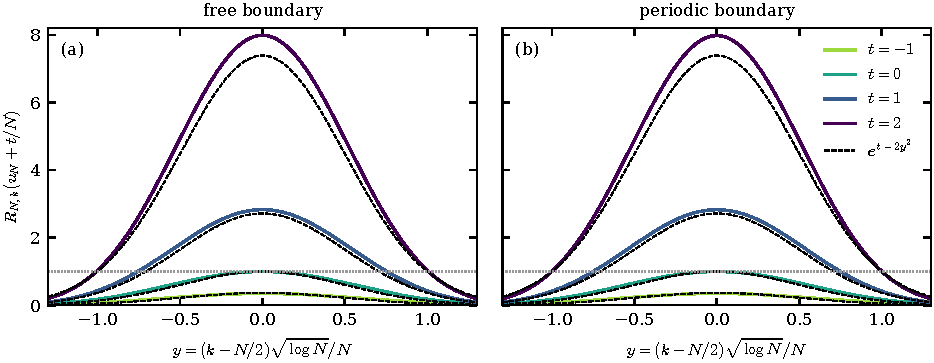
\includegraphics{figures/window}
\caption{The exact ratios $R^X_{N,k}(u_N^X+t/N)$ at $N=10^6$ for free (a) and
periodic (b) boundaries, with the limit $e^{t-2y^2}$ of
Theorem~\ref{thm:critical-window} (dashed). Here $y=(k-N/2)\sqrt{\log N}/N$,
and the bins above the dotted line are above the endpoint height. The
convergence is slow, and at $t=2$ and $y=0$ the relative error is still $0.08$.}
\label{fig:window}
\end{figure}
